\chapter{Risultati della calibrazione}
In questo capitolo ci si occupa dell'analisi degli scostamenti fra simulazione numerica e dati ematici, a seguito della scelta di utilizzare un modello calibrato su tre parametri (\textsection\ref{sec:calibrazione}). Si è cercato di evidenziare gli aspetti rilevanti, rivolgendo particolare attenzione ai soluti la cui concentrazione plasmatica reale si discosta maggiormente dalla simulazione numerica.

Tramite il comando \verb|boxplot| di matlab è possibile ottenere una visione generale e immediata della distibuzone degli scostamenti per ogni singolo soluto.
\begin{figure}[htb]
	\centering
	\advance\leftskip-.1\textwidth
		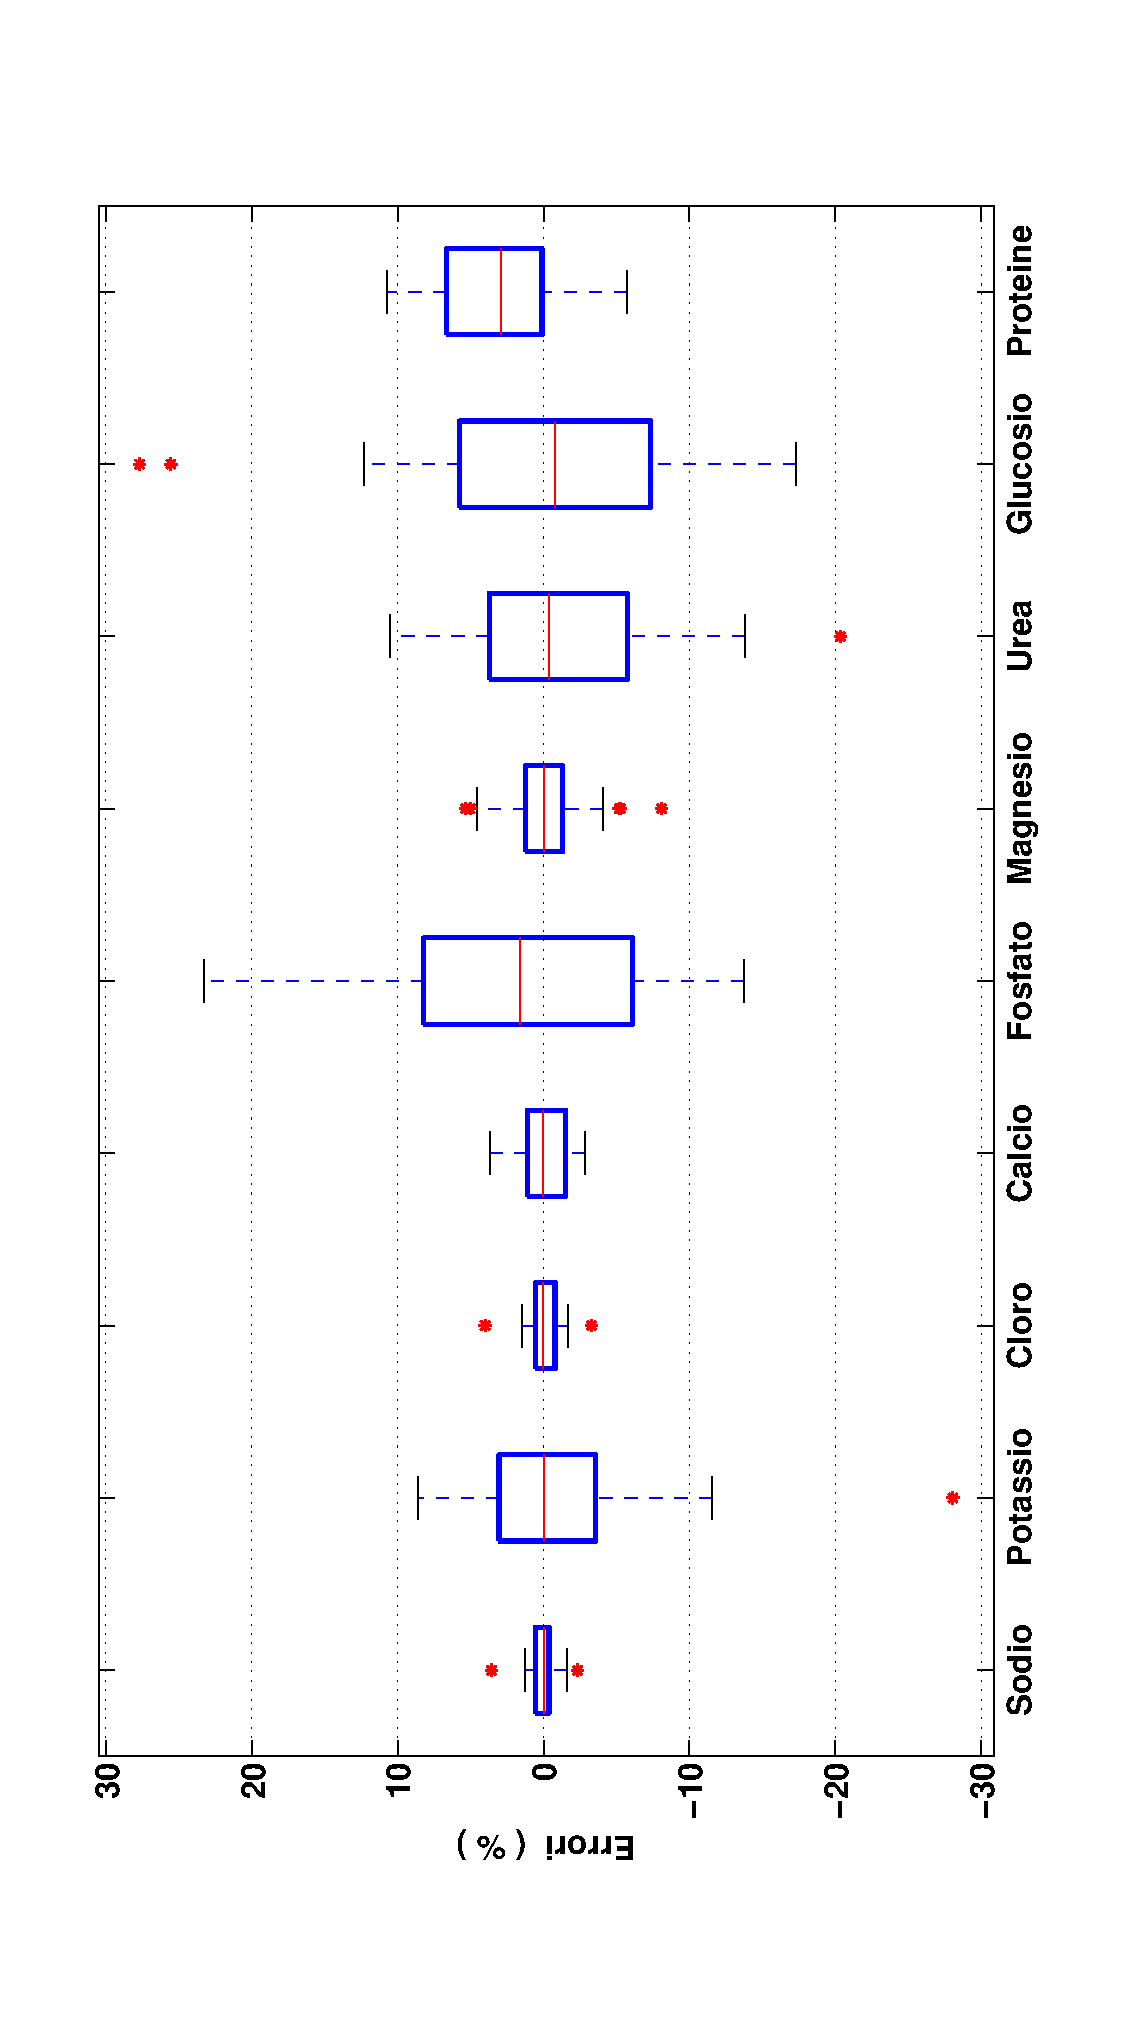
\includegraphics[angle=-90, width=1.2\textwidth]{immagini/boxplot_calibrazione.eps}
		\caption{Boxplot degli scostamenti percentuali calcolati con l'Eq.(\ref{eq:Epercent}) della simulazione numerica calibrata su tre parametri.}
		\label{fig:boxplot}
\end{figure}
In generale, oltre il $50\%$ degli scostamenti si situa nella fascia d'errore del $\pm 10\%$. Gli errori si riducono ulteriormente se si considerano gli ioni sodio, cloro, calcio e magnesio. Si dà ora una descrizione dettagliata per ogni soluto del comportamento degli errori di simulazione, individuando dei possibili motivi che giustifichino la presenza di \textit{outlier} nella \figurename\ref{fig:boxplot}.

\begin{description}
	\item[Sodio:] tutti gli errori, \textit{outlier} compresi, sono contenuti nella fascia del $\pm 5\%$. Tolti i due \textit{outlier} ($+3,57\%$ per il paziente AMB e $-2,34\%$ per il paziente SIM), gli scostamenti risultano compresi nella fascia del $\pm 2\%$.
	\item[Potassio:] gli errori sono distribuiti più ampiamente rispetto al sodio, con un \textit{outlier} pari a $-28,6\%$ (paziente AMB). Probabilmente la causa di questi errori non è da ricercare nella modellizzazione, ma piuttosto nell'emolisi generatasi per il metodo di conservazione del campione (congelamento a $-30\degree C$): il potassio, altamente concentrato nei globuli rossi, potrebbe essere stato rilasciato nel plasma, inficiando quindi le misure effettuate dopo lo scongelamento. Un caso particolarmente anomalo è costituito dal paziente AMB (\figurename\ref{fig:ambcal}), nel quale il potassio aumenta durante il corso della dialisi, a differenza di tutti gli altri pazienti in cui diminuisce sempre. Per questo paziente bisognerà ripetere le analisi.
	\item[Cloro:] analogamente al sodio, il cloro presenta una fascia d'errore del $\pm 5\%$ con due \textit{outlier} ($-3,29\%$ per AMB; $+4,01\%$ per SIM).
	\item[Calcio:] anche per il calcio la fascia d'errore e del $\pm 5\%$. Non ci sono \textit{outlier}.
	\item[Fosfato:] questo è il soluto che risulta più disperso e che globalmente rende gli errori di simulazione non inferiori al $20\%$. Infatti i valori degli scostamenti percentuali superano la fascia del $\pm 10\%$ fino a punte del $23,28\%$. La causa può essere attribuita alla modellizazione della cinetica del soluto. Infatti, nella letteratura medica \cite{bib:fosfato} il fosfato plasmatico, durante il corso della dialisi, presenta un andamento bifasico decrescente/crescente, tale per cui se la concentrazione del fosfato scende al di sotto di una certa soglia, entra in azione un meccanismo che tende a farne rialzare la concentrazione plasmatica. Effettivamente possiamo constatare che in alcuni pazienti (EAS, GRA, LI, ZAN), la concentrazione a fine dialisi del fosfato è superiore rispetto alla rilevazione precedente. Per ridurre gli errori nella simulazione, bisognerebbe introdurre un ulteriore compartimento specifico per tale soluto.
	\item[Magnesio:] per questo ione si hanno scostamenti del $\pm 5\%$, eccezione fatta per il valore della prima rilevazione del paziente LI, che risulta essere pari a $-8,10\%$.
	\item[Urea:] gli errori sono contenuti nella fascia del $\pm 15\%$ (ad eccezione di AMB: $-20,35\%$). Rispetto allo ione sodio, gli errori sull'urea hanno una distribuzione più ampia. Questo potrebbe essere dovuto all'uso dell'Eq.(\ref{eq:Epercent}) per il calcolo delgi errori: il denominatore dell'equazione è più grande per il sodio (circa $140$ $mmol/L$) che per l'urea (circa $15$ $mmol/L$), rendendo di conseguenza, a parità dello stesso scosatmento in $mmol/L$, più grande l'errore relativo percentuale nella simulazione dell'urea.
	\item[Glucosio:] la maggior parte gli errori commessi simulando il glucosio sono contenuti nella fascia del $\pm 20\%$. La loro distribuzione è più ampia rispetto a quella del sodio perché il modello non tiene conto degli spuntini che i pazienti sono soliti effettuare dopo la prima ora, che alterano senz'altro l'andamento della glicemia (GAR, LI). Qualora, per limitare gli errori, si introducesse nel modello un termine di generazione del glucosio non nullo, sarebbe comunque difficile quantificare gli zuccheri e carboidrati ingeriti. Ulteriore difficoltà di modellizzazione del glucosio è data dalla presenza in dialisi di pazienti diabetici.
	\item[Proteine:] si nota subito che, a differenza di tutti gli altri soluti, le proteine presentano sugli errori una mediana più alta. Sembrerebbe che il modello tenda a sovrastimare il contenuto plasmatico delle proteine, ma ciò potrebbe anche essere dovuto al metodo di preparazione dei campioni da analizzare. Prima di centrifugare i campioni bisognerebbe attendere almeno un'ora\footnote{in teoria basterebbe attendere mezz'ora, ma dato che i pazienti in dialisi sono solitamente sotto anticoagulanti, sarebbe meglio attendere di più.} dal prelievo, per consentire il ritiro e la formazione del coagulo. Se il campione viene centrifugato, come invece è stato fatto, immediatamente dopo il prelievo, accade che, dopo la centrifugazione, nella frazione di plasma si forma un coagulo di fibrina che può sequestrare le proteine. Il macchinario che esegue le analisi del sangue, usando solo la parte liquida del plasma, potrebbe fornire misure che sottostimino l'effettivo contenuto proteico contenuto originariamente nel campione.
\end{description}

Gli errori più grandi riguardano il paziente AMB, per il quale bisognerà ripetere le misurazioni. Tali errori potrebbero essere stati indotti dall'emolisi e/o dalla centrifugazione precoce del campione, e non si esclude che ciò abbia coinvolto anche le misurazioni degli altri pazienti.

\begin{figure}[htb]
	\centering
	\advance\leftskip-.2\textwidth
		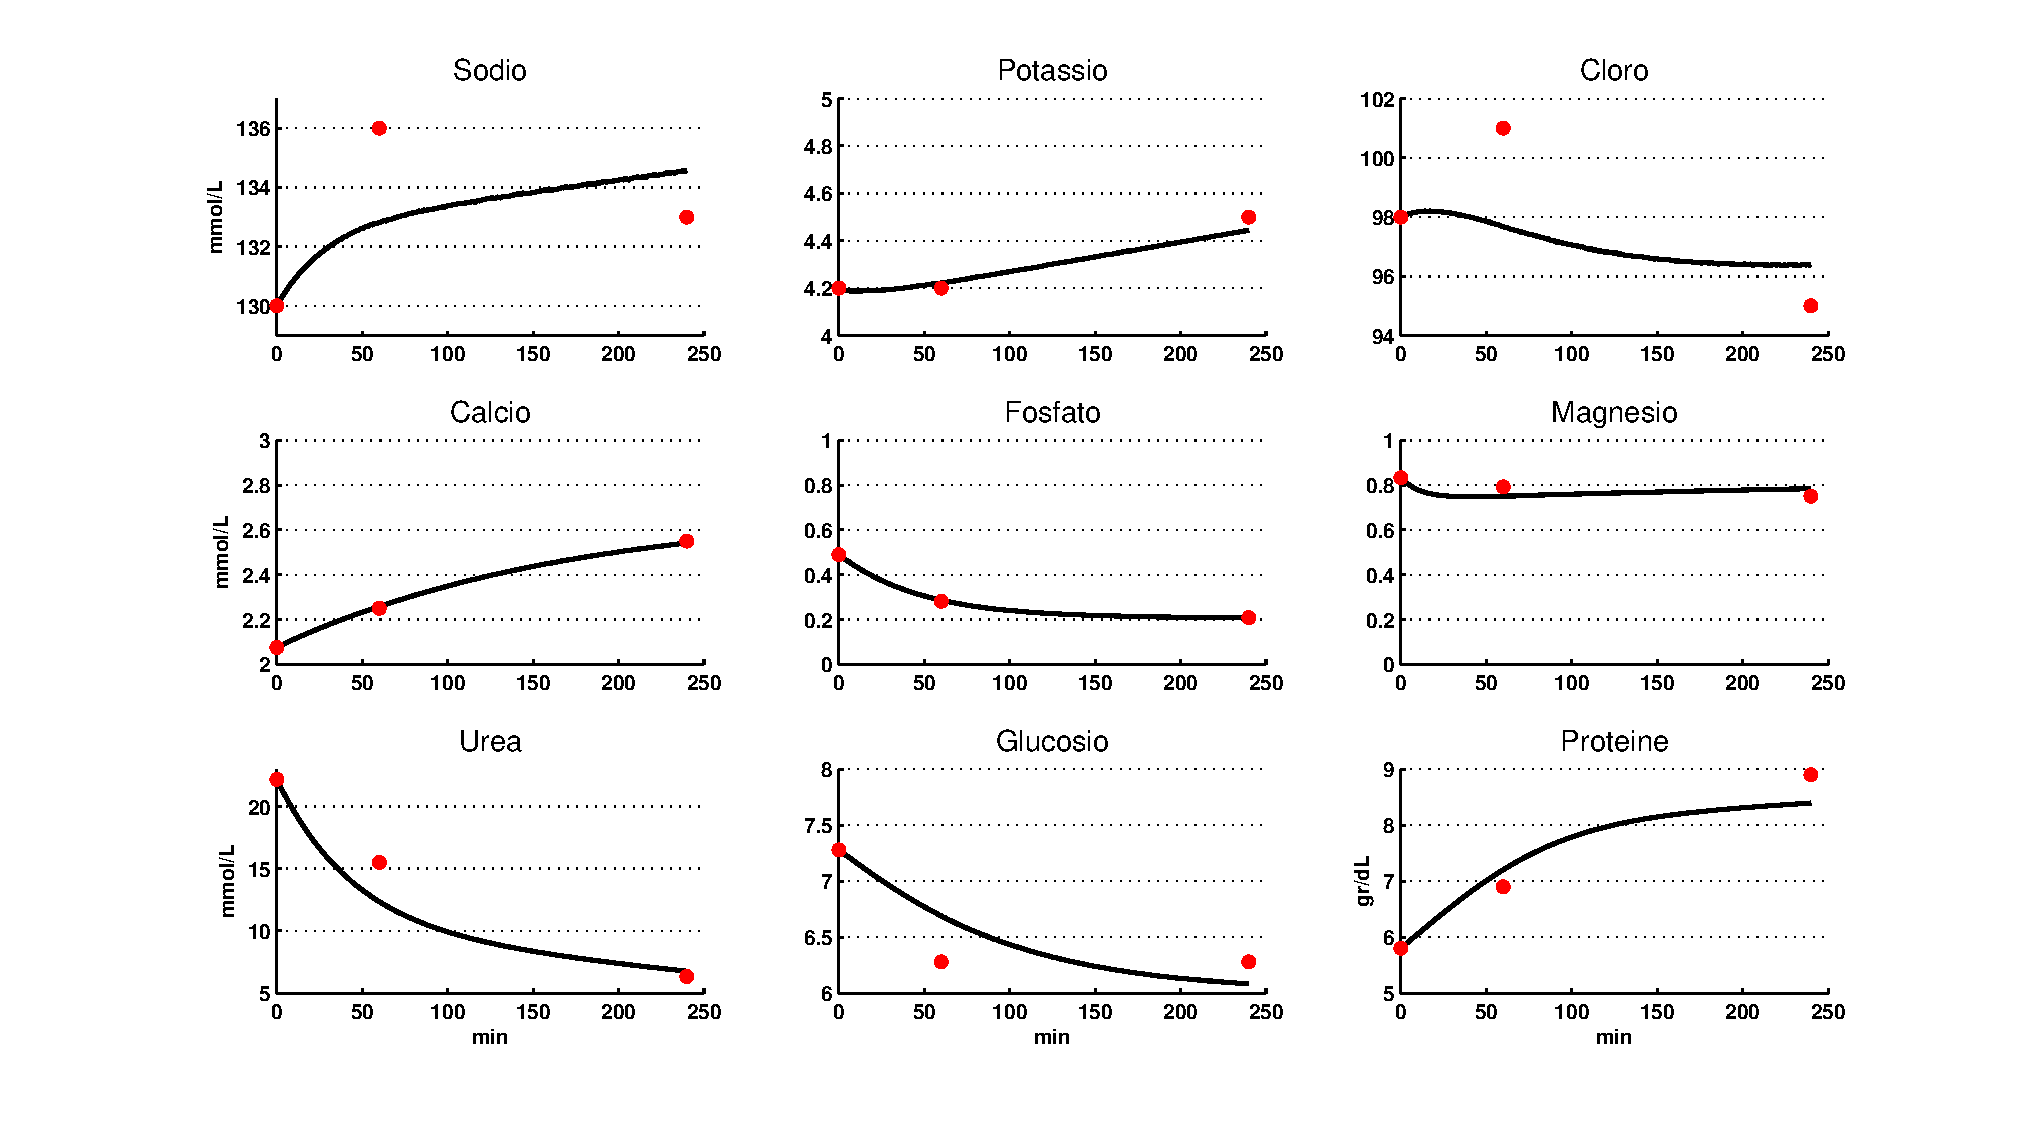
\includegraphics[width=1.4\textwidth]{immagini/ambcal.eps}
		\caption{paz. AMB}\label{fig:ambcal}		
\end{figure}
\begin{figure}[htb]
	\centering
	\advance\leftskip-.2\textwidth
		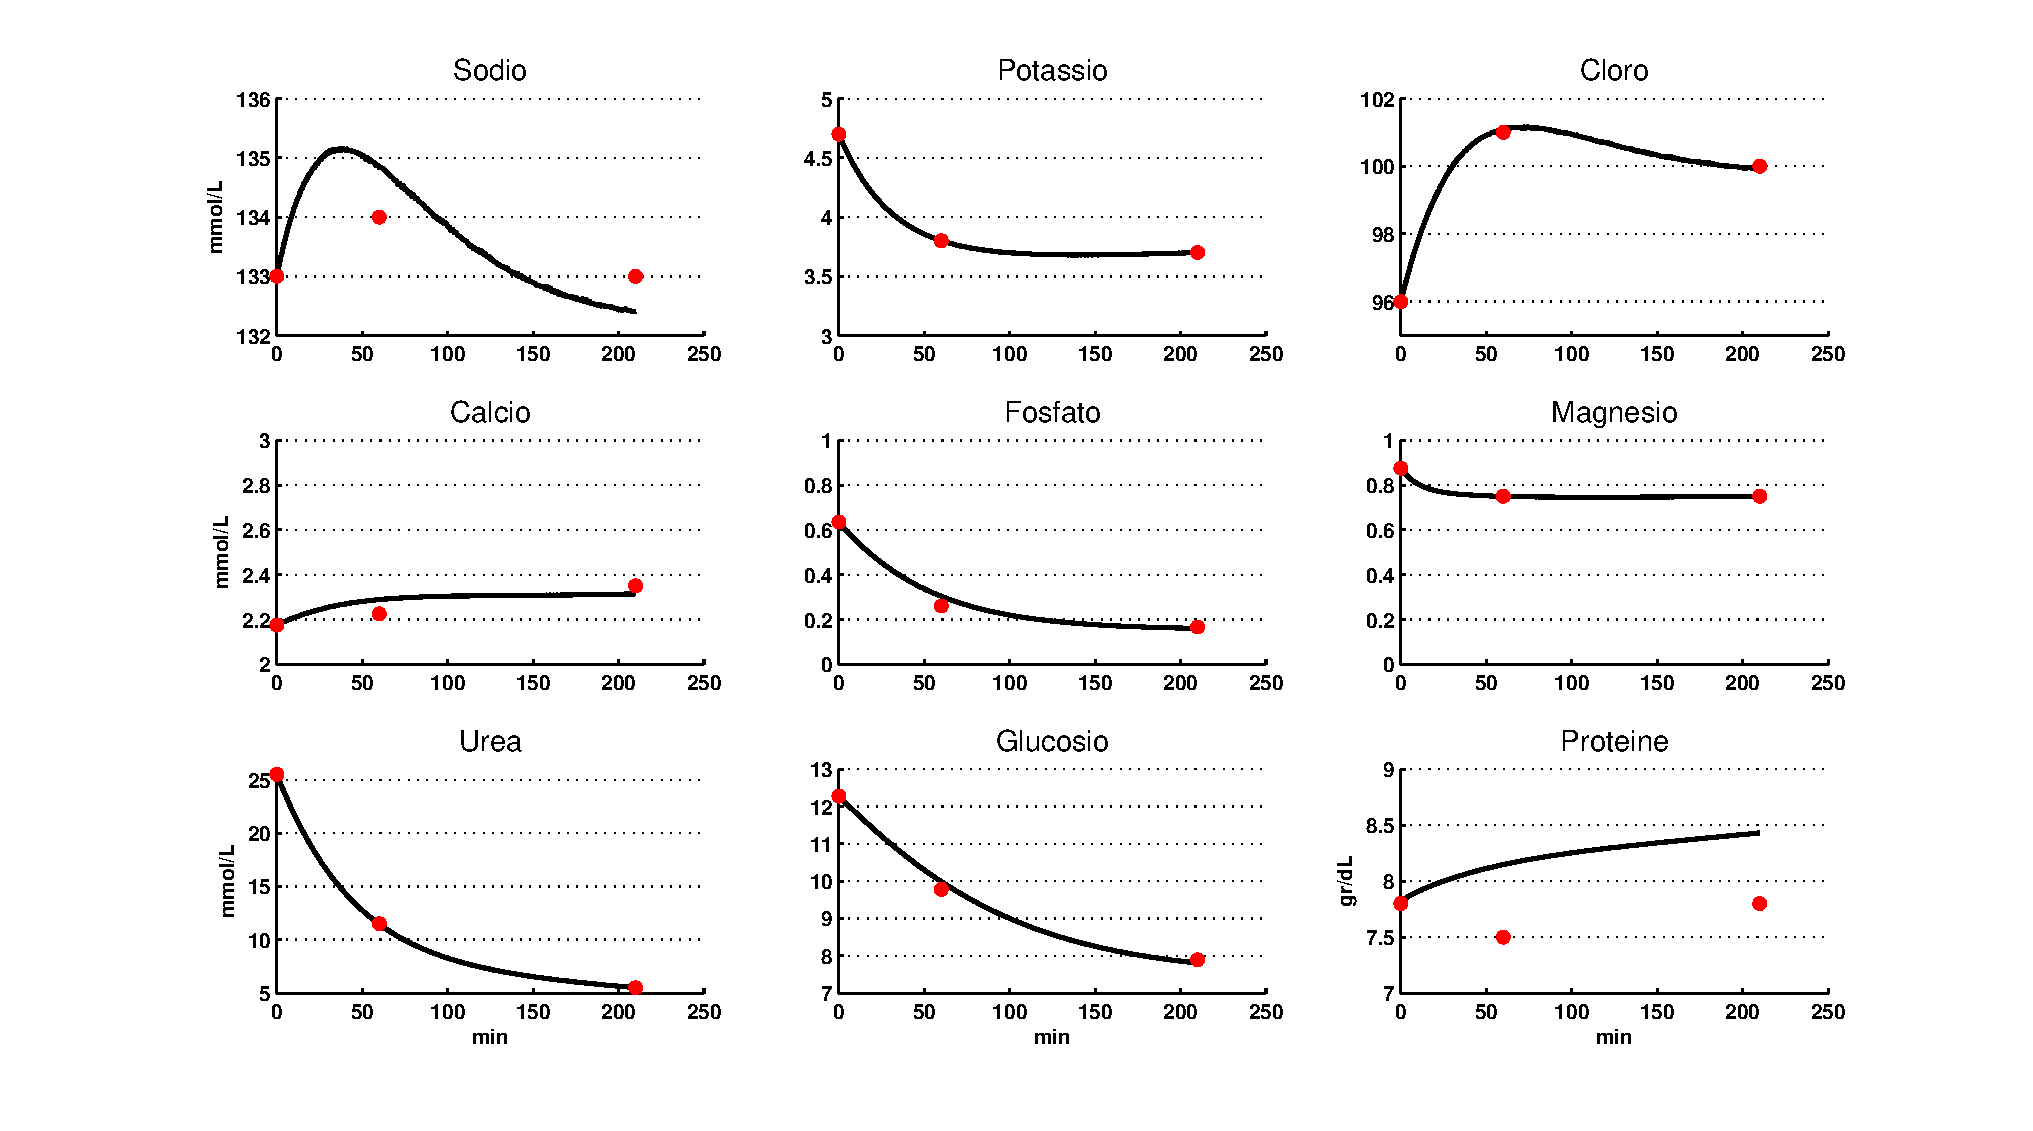
\includegraphics[width=1.4\textwidth]{immagini/betcal.eps}
		\caption{paz. BET}		
\end{figure}
\begin{figure}[htb]
	\centering
	\advance\leftskip-.2\textwidth
		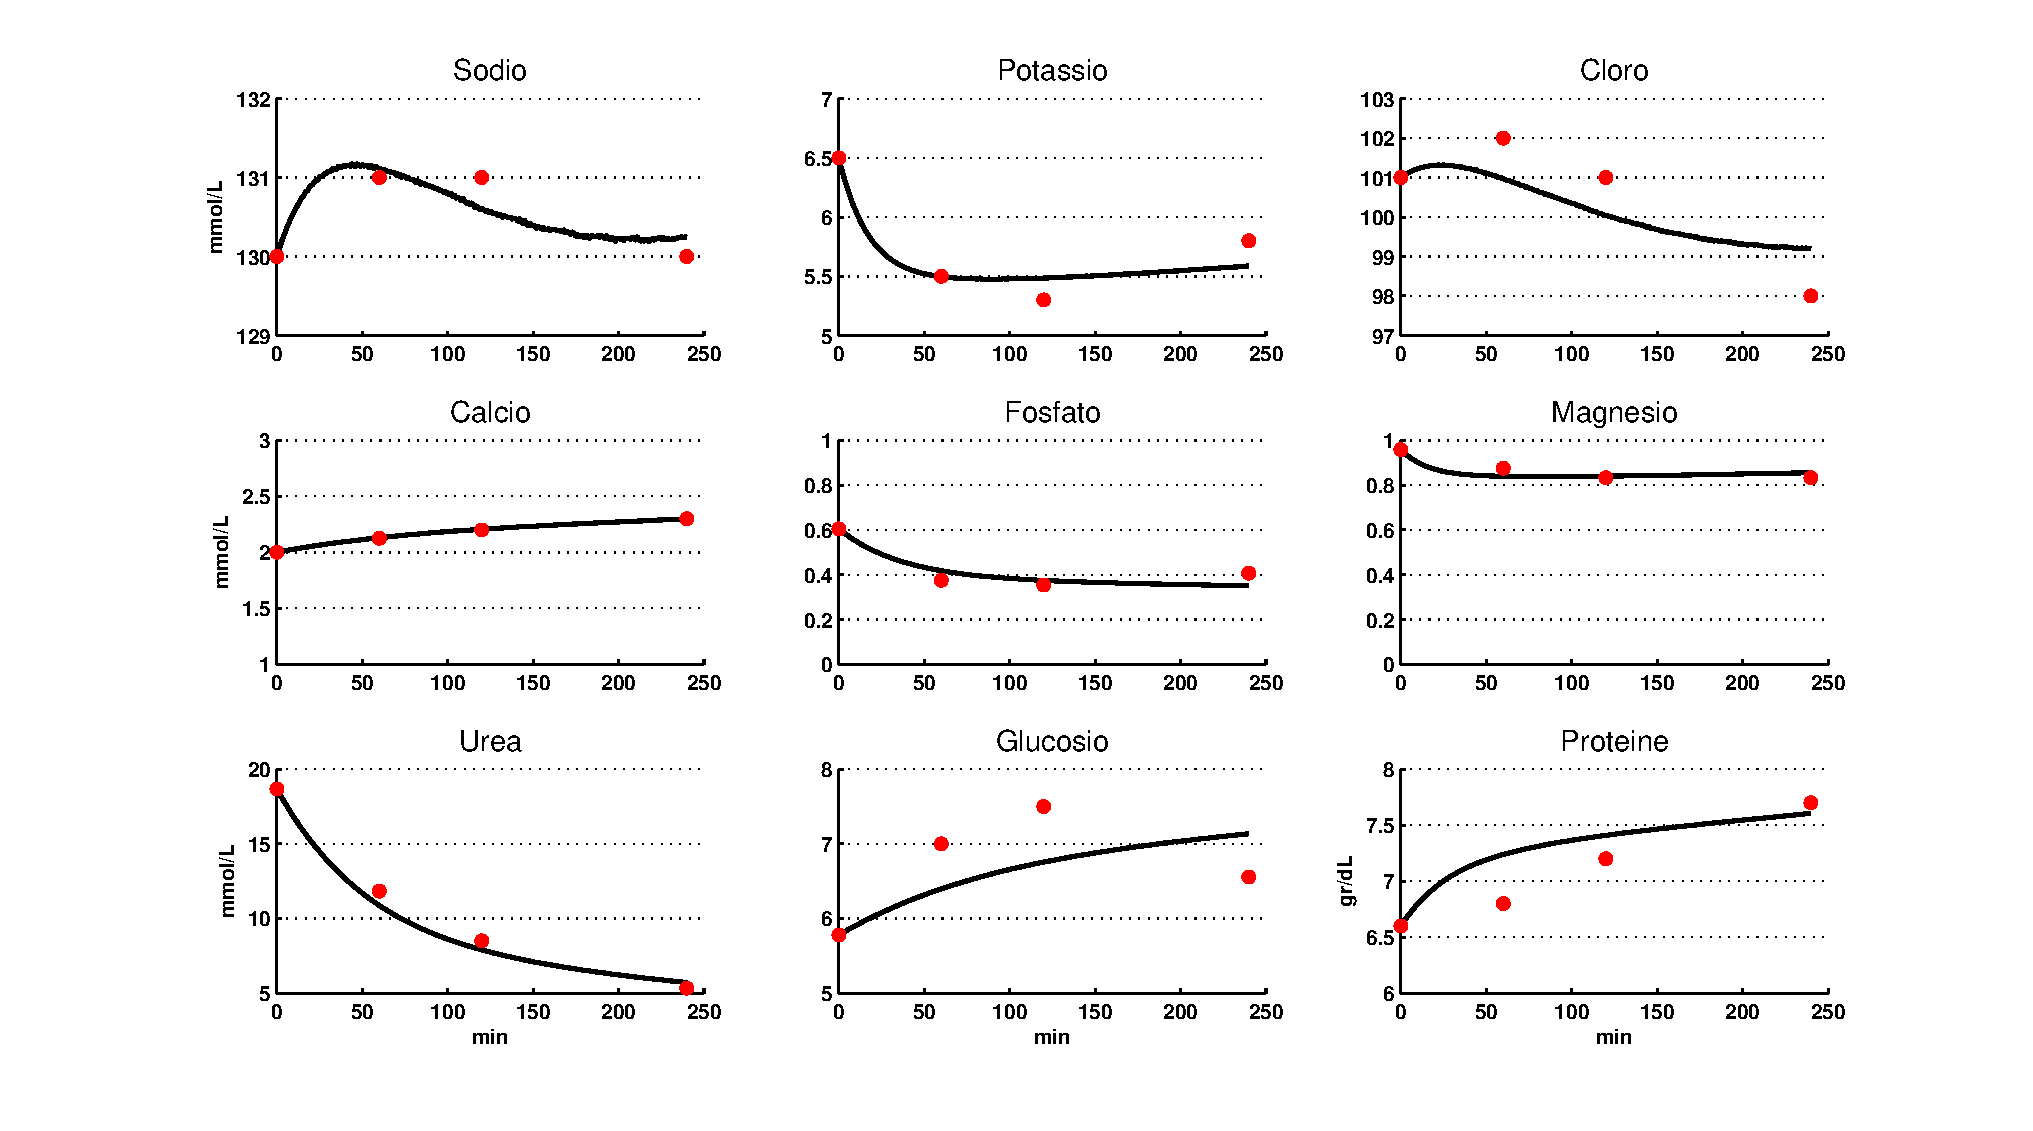
\includegraphics[width=1.4\textwidth]{immagini/eascal.eps}
		\caption{paz. EAS}		
\end{figure}
\begin{figure}[htb]
	\centering
	\advance\leftskip-.2\textwidth
		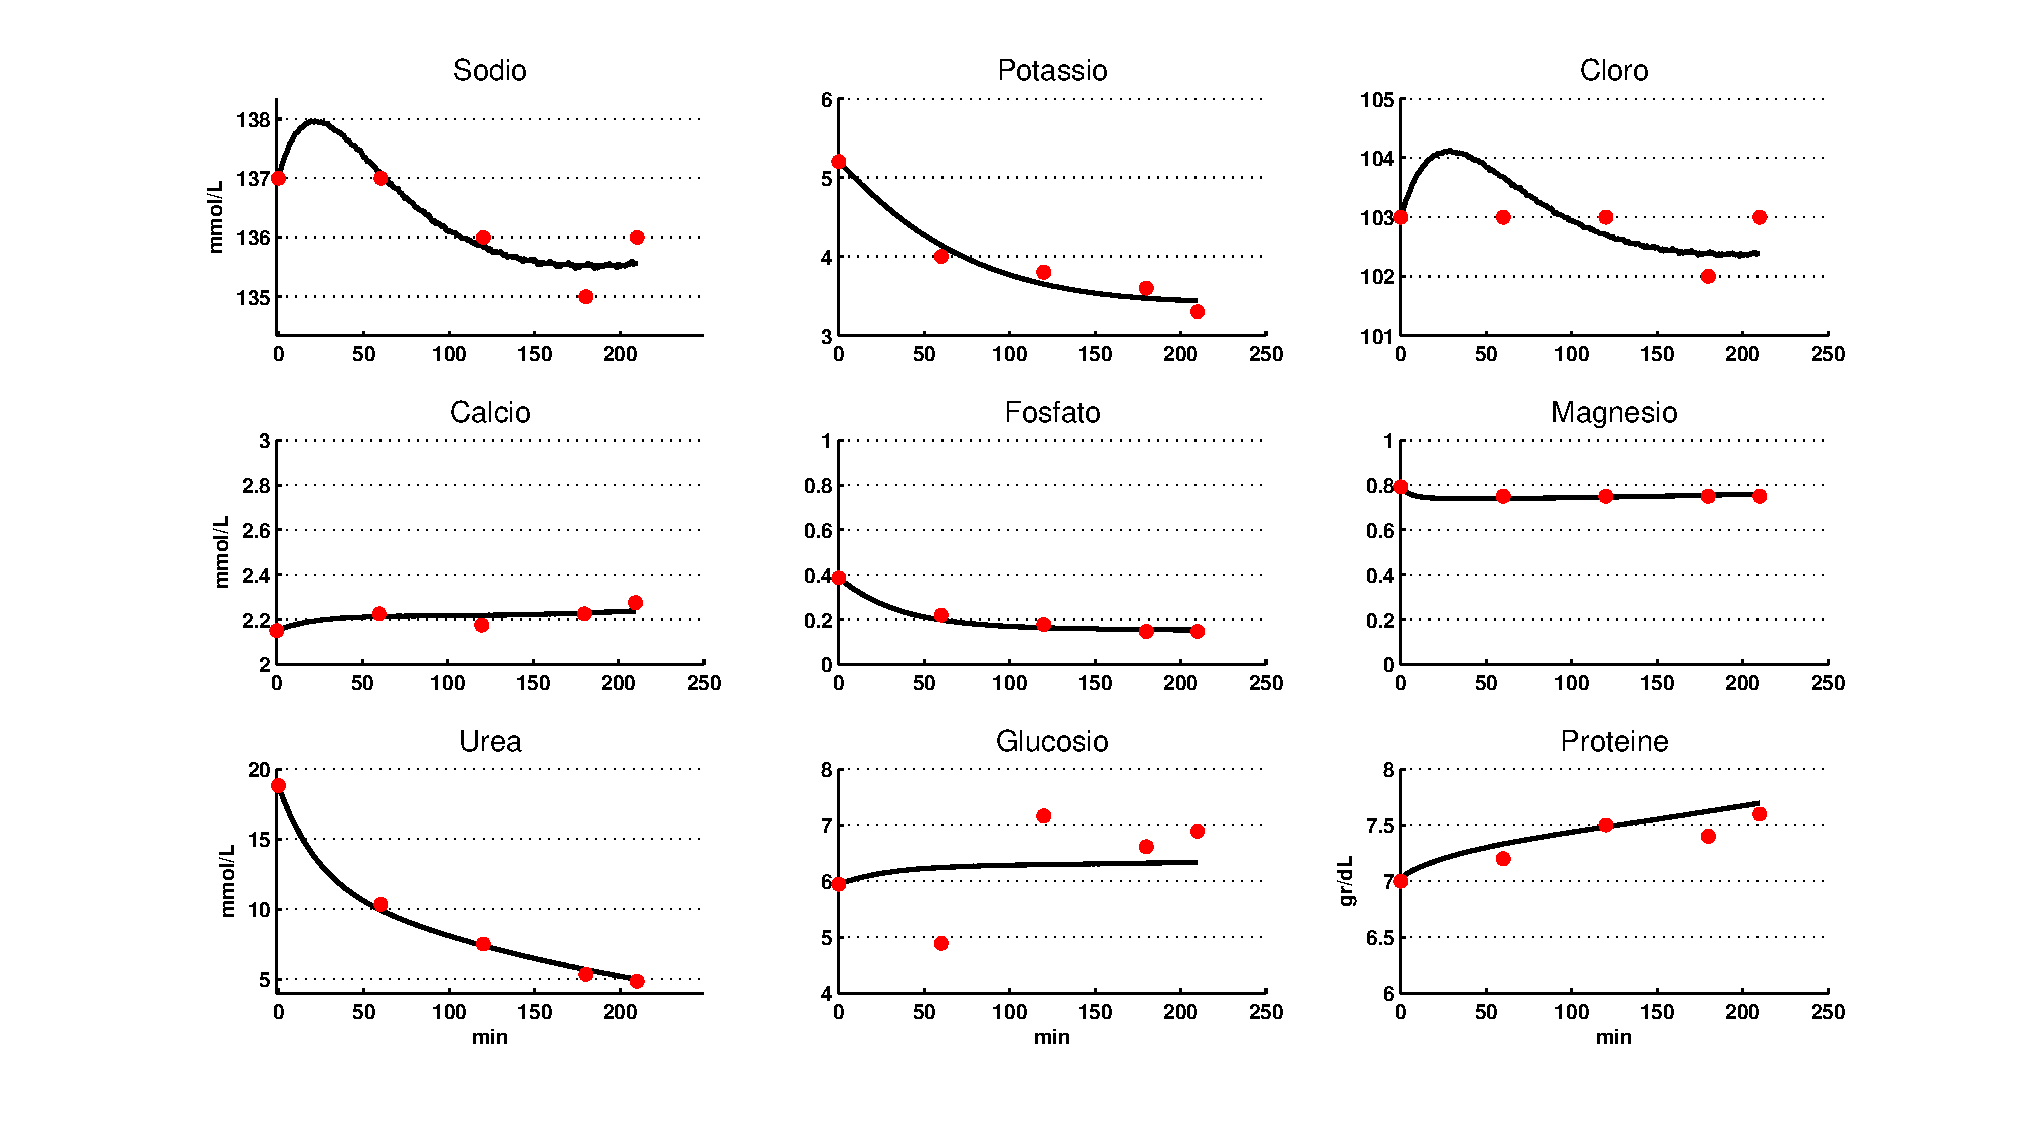
\includegraphics[width=1.4\textwidth]{immagini/garcal.eps}
		\caption{paz. GAR}		
\end{figure}
\begin{figure}[htb]
	\centering
		\advance\leftskip-.2\textwidth
		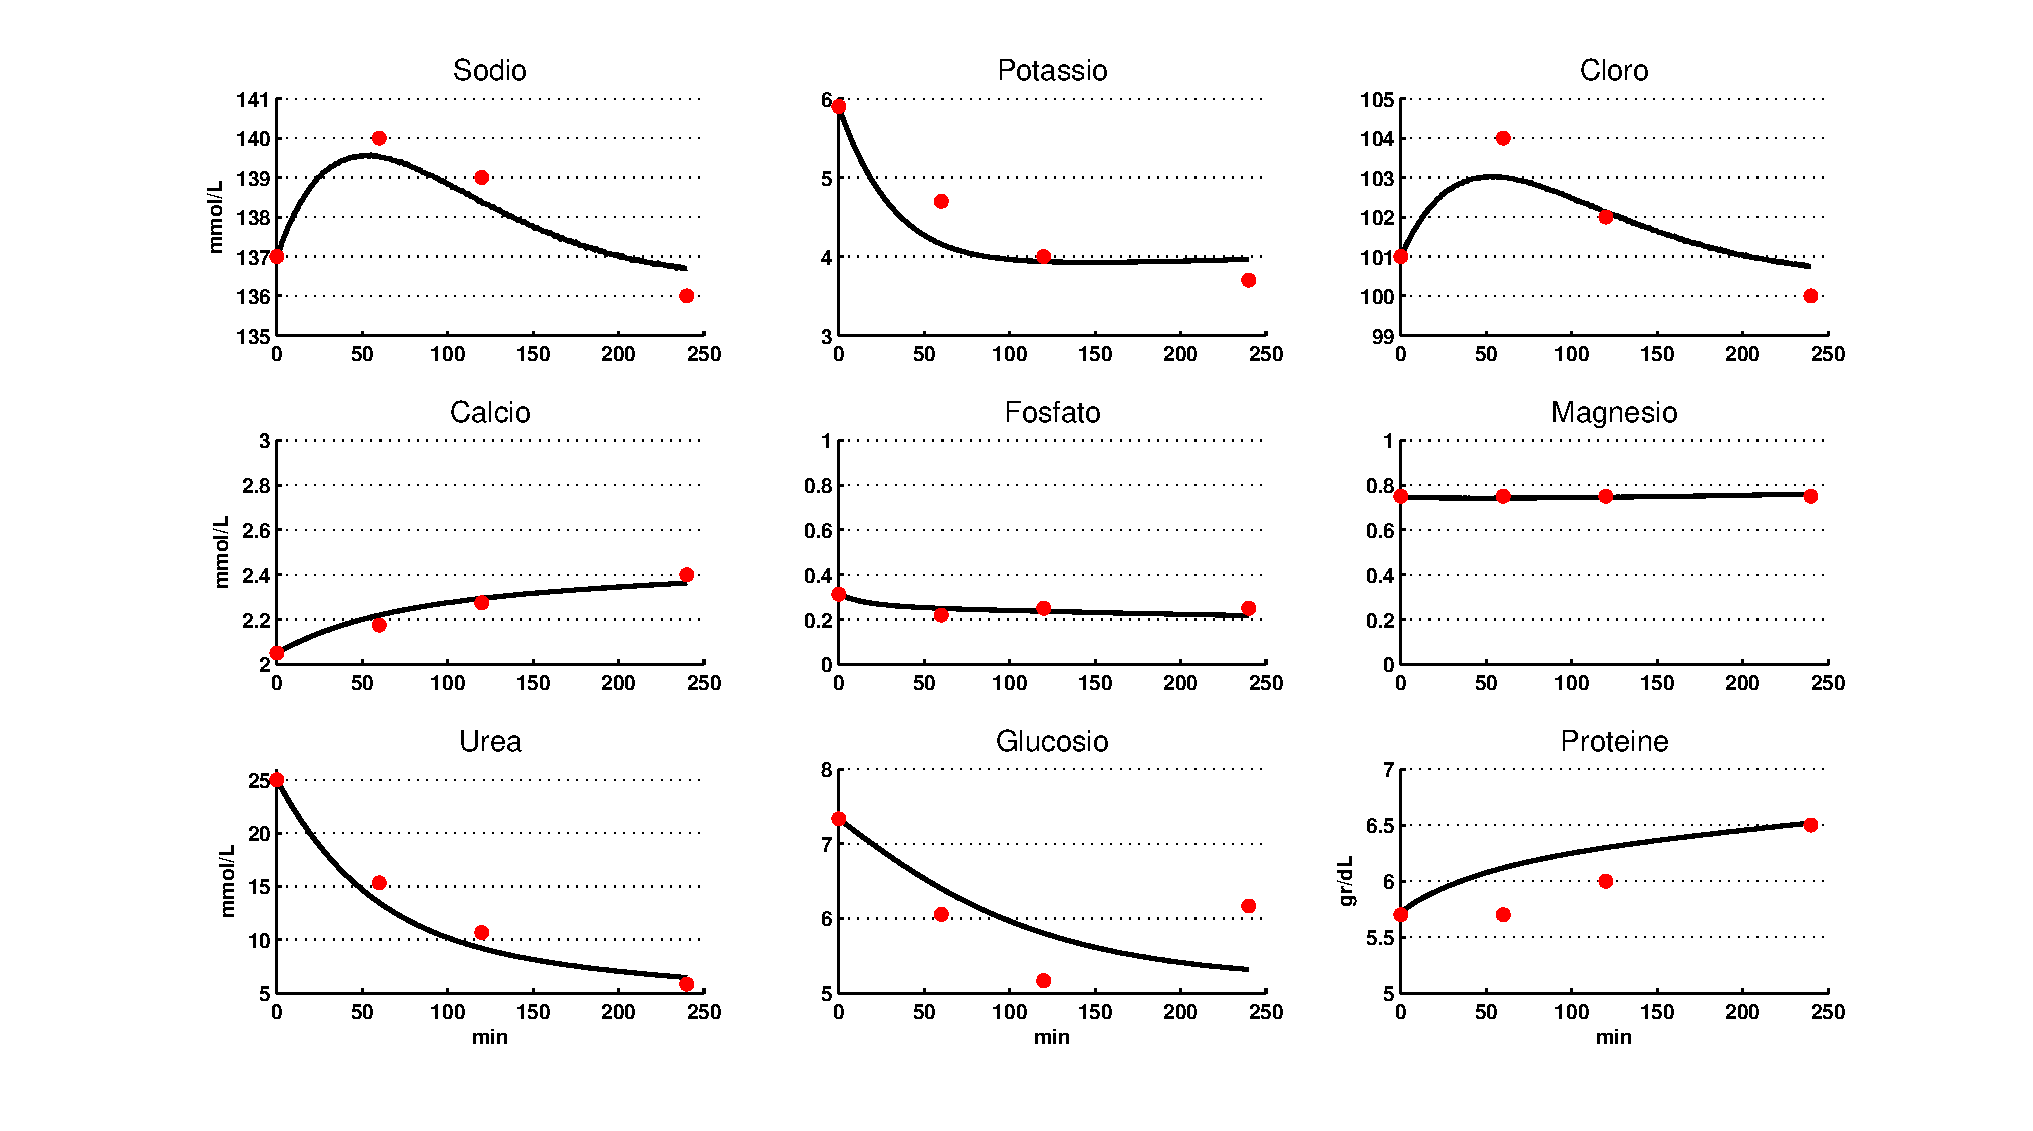
\includegraphics[width=1.4\textwidth]{immagini/gracal.eps}
		\caption{paz. GRA}		
\end{figure}
\begin{figure}[htb]
	\centering
		\advance\leftskip-.2\textwidth
		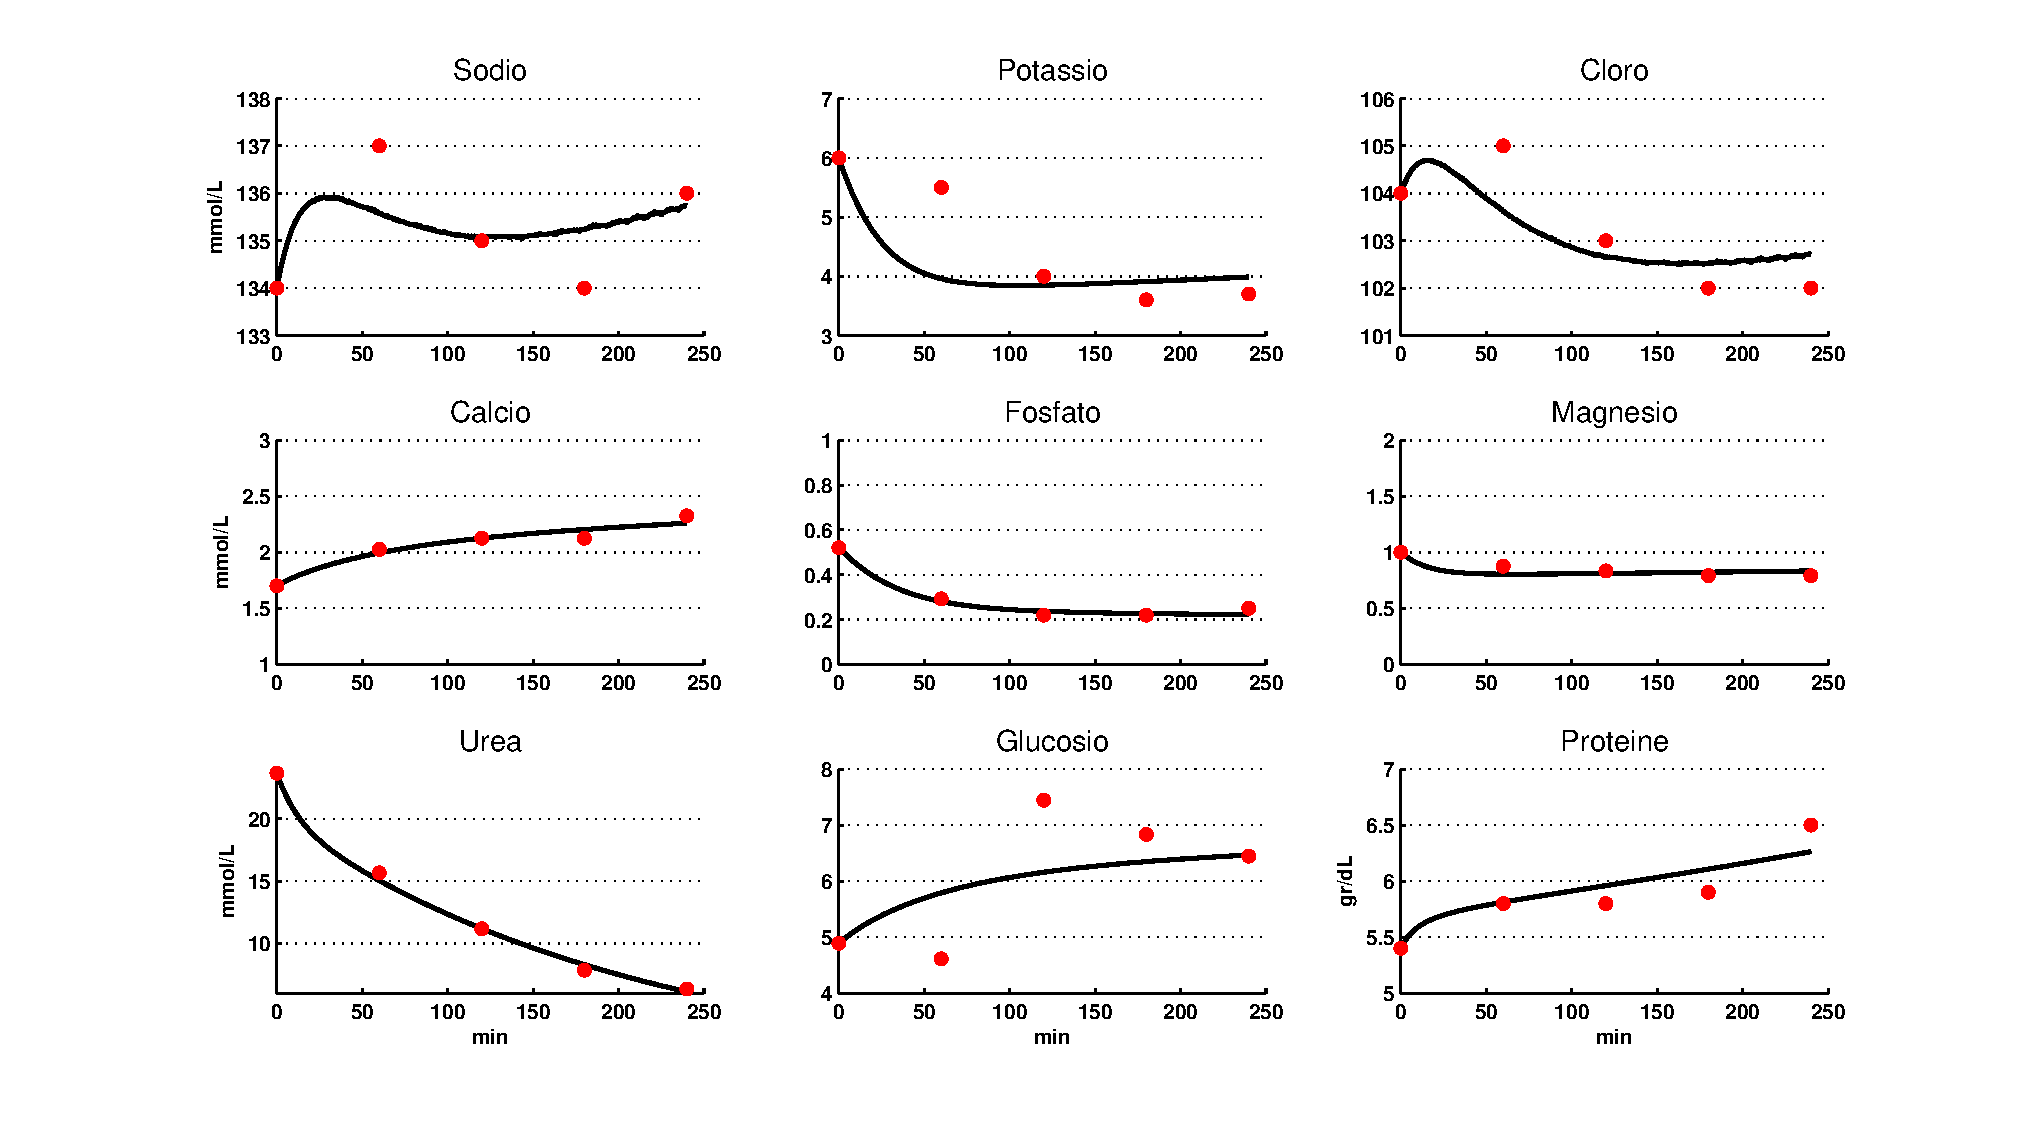
\includegraphics[width=1.4\textwidth]{immagini/lical.eps}
		\caption{paz. LI}		
\end{figure}
\begin{figure}[htb]
	\centering
		\advance\leftskip-.2\textwidth
		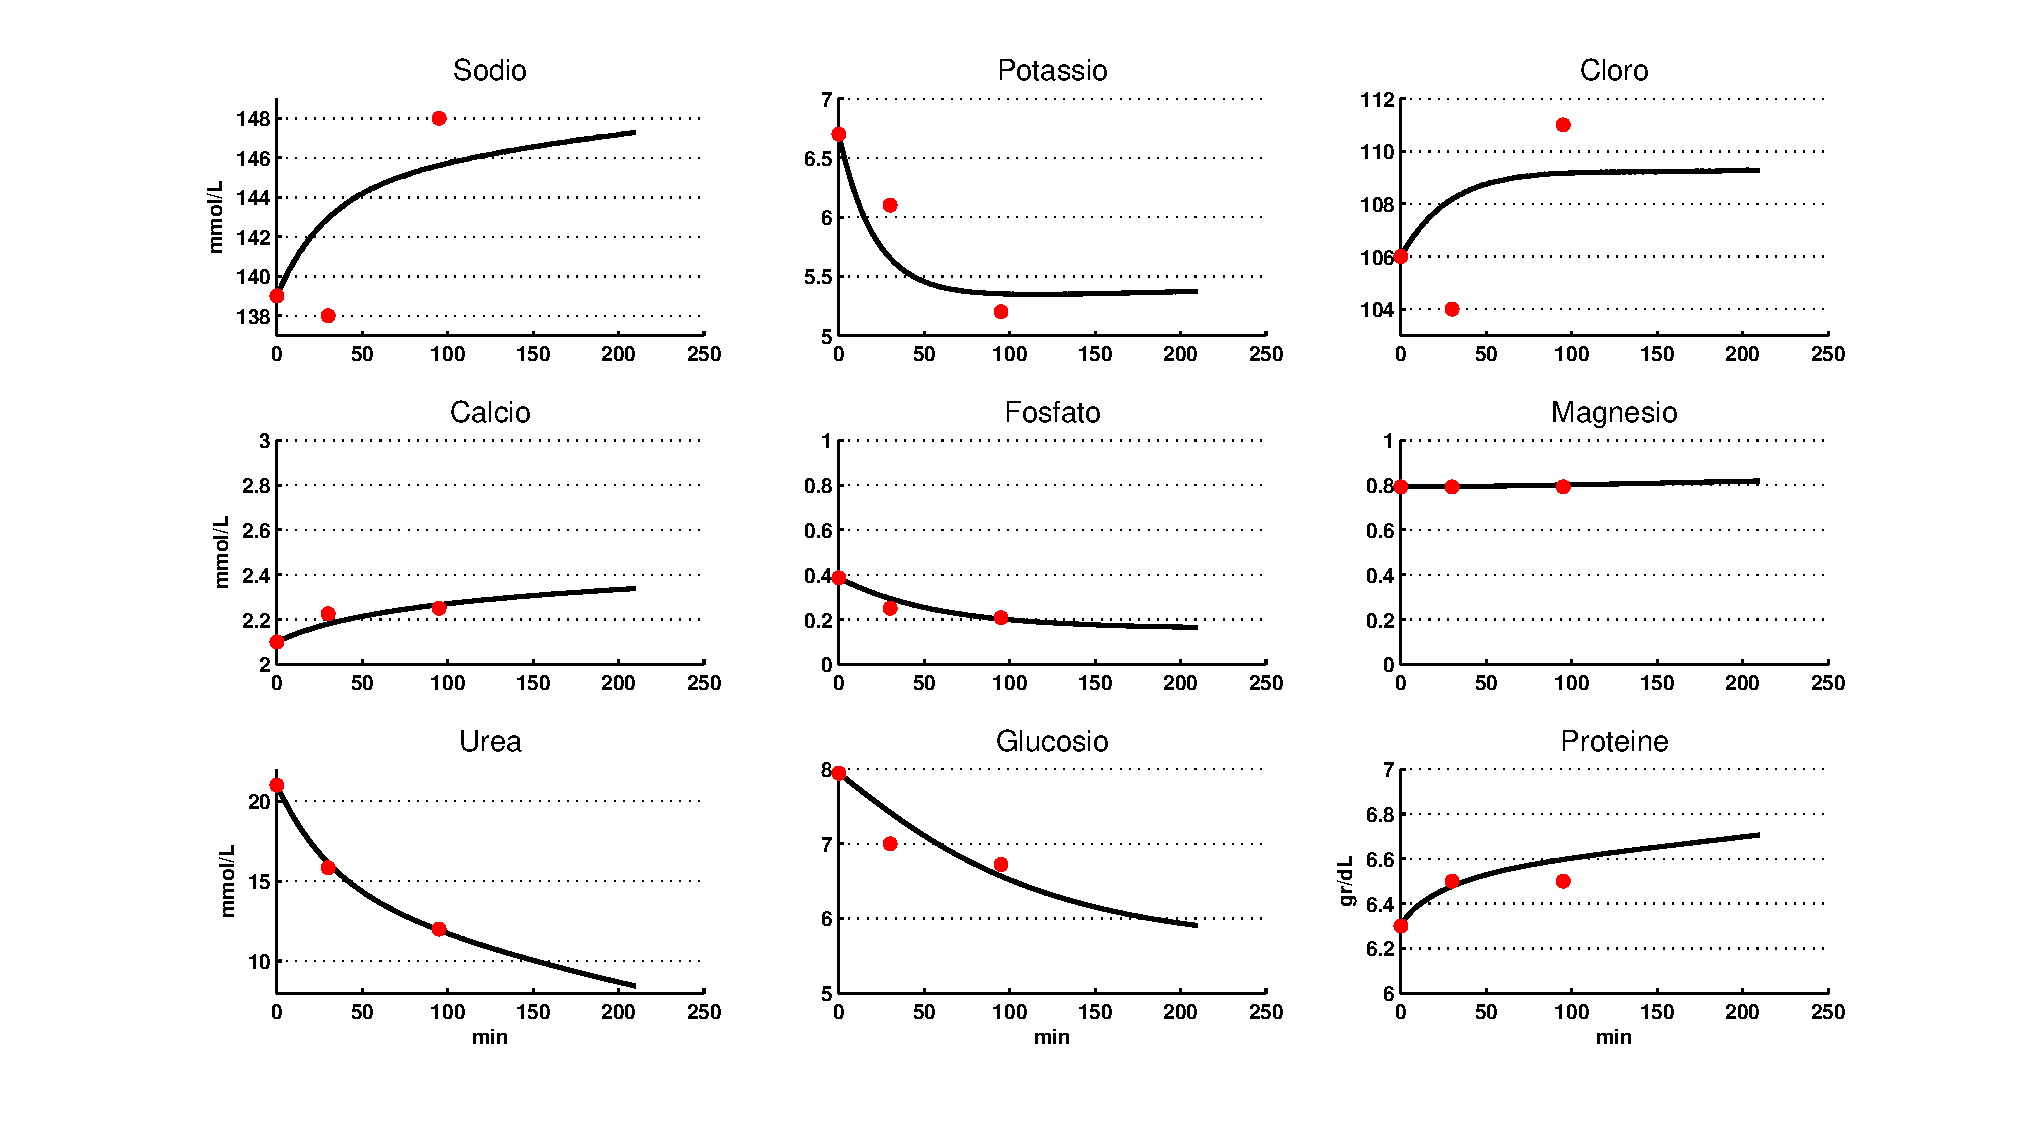
\includegraphics[width=1.4\textwidth]{immagini/simcal.eps}
		\caption{paz. SIM}		
\end{figure}
\begin{figure}[htb]
	\centering
		\advance\leftskip-.2\textwidth
		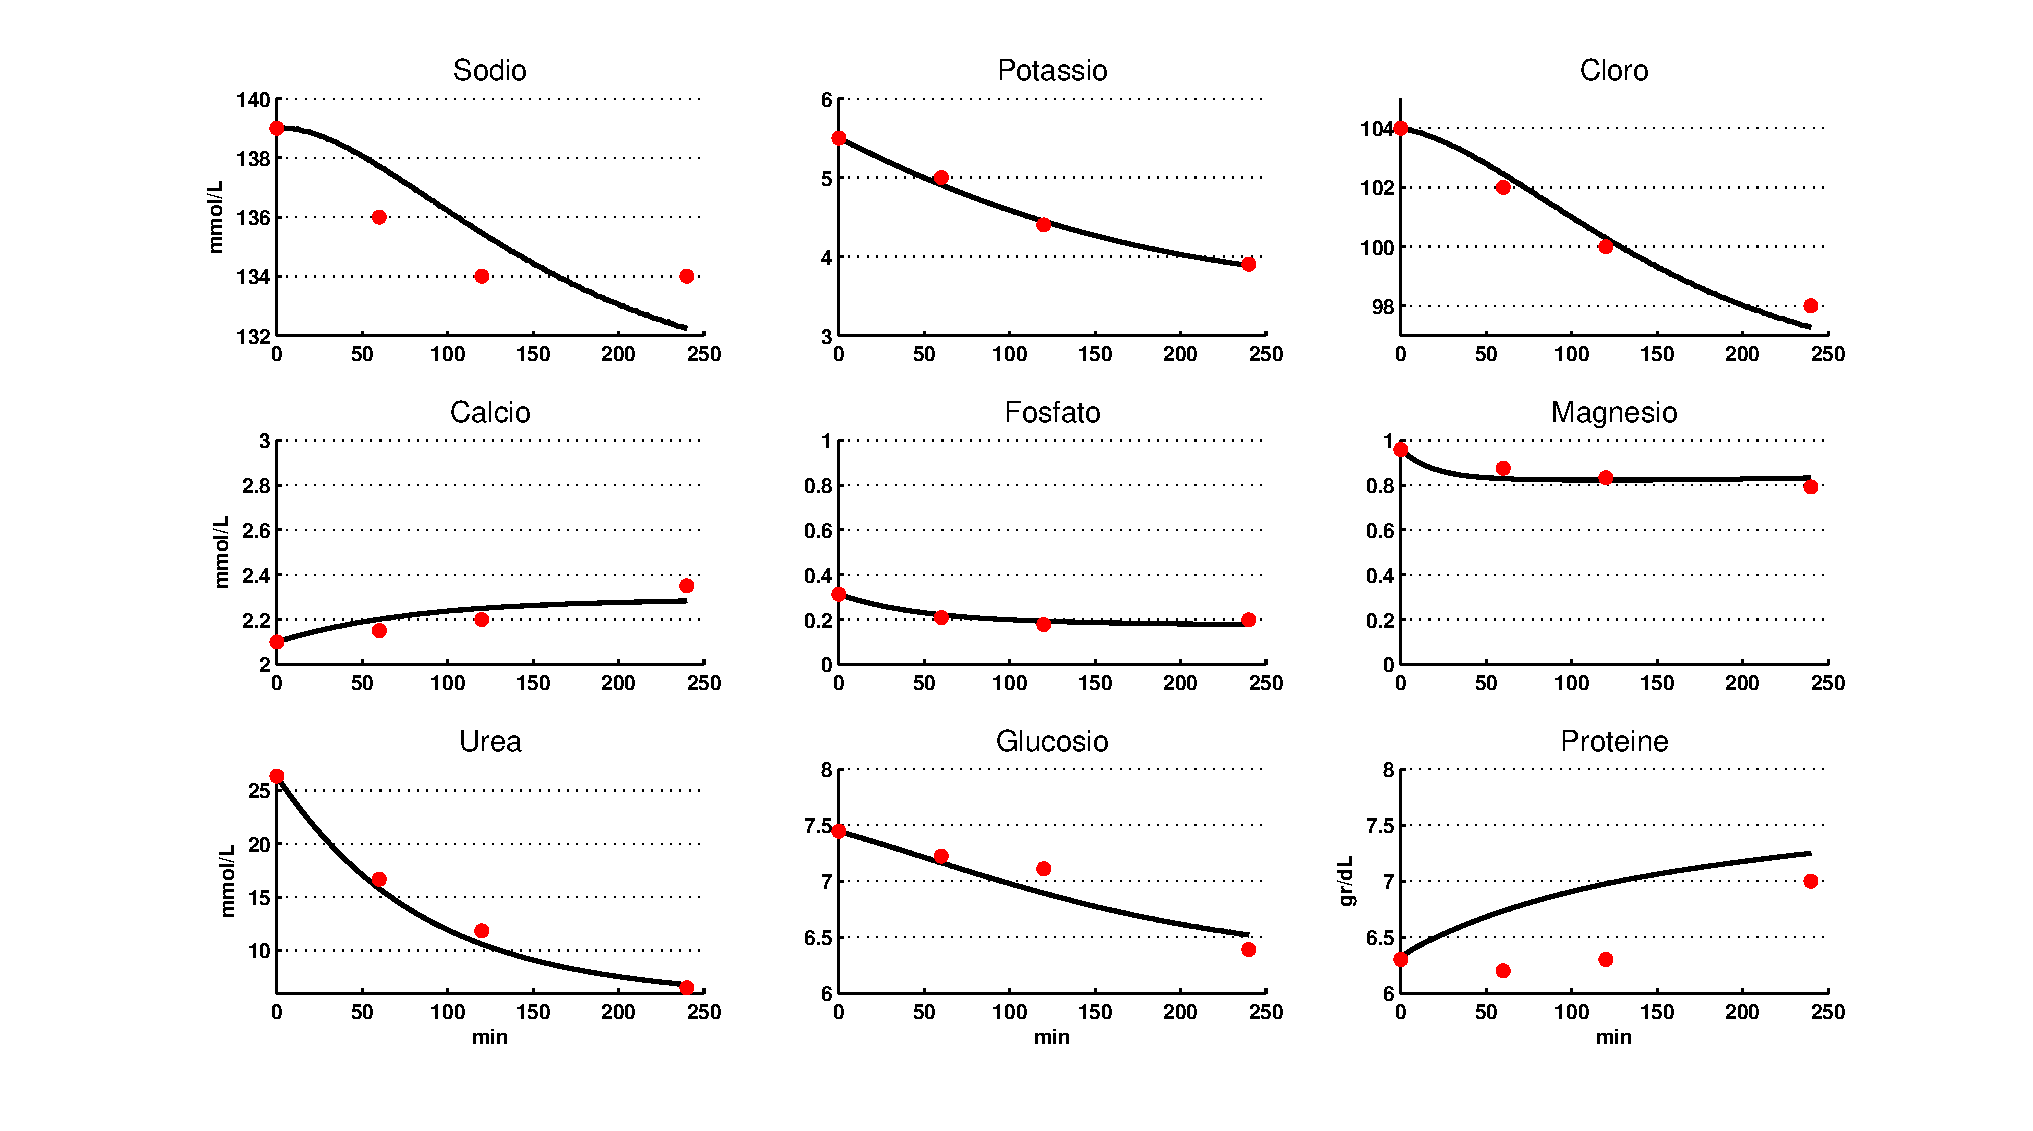
\includegraphics[width=1.4\textwidth]{immagini/zancal.eps}
		\caption{paz. ZAN}		
\end{figure}